\documentclass[12pt]{article}
\usepackage{url,graphicx,tabularx,array}
\usepackage[margin=1in]{geometry}
\setlength{\parskip}{1ex} %--skip lines between paragraphs
\setlength{\parindent}{0pt} %--don't indent paragraphs

\usepackage{algorithmic}
\usepackage{algorithm}
\usepackage{ amssymb }
\usepackage{ latexsym }
\usepackage{ amsmath }
\usepackage{ amsthm }
%-- Commands for header
\renewcommand{\title}[1]{\textbf{#1}\\}
\renewcommand{\line}{\begin{tabularx}{\textwidth}{X>{\raggedleft}X}\hline\\\end{tabularx}\\[-0.5cm]}
\newcommand{\leftright}[2]{\begin{tabularx}{\textwidth}{X>{\raggedleft}X}#1%
& #2\\\end{tabularx}\\[-0.5cm]}

\newtheorem{defn}{Definition}[section]
\newtheorem{conjecture}{conjecture}[section]
\newtheorem{lemma}{Lemma}[section]
\newtheorem{corollary}{Corollary}[section]
\newtheorem{question}{Question}[section]
\newtheorem{proposition}{Proposition}[section]


%\linespread{2} %-- Uncomment for Double Space
\begin{document}

\title{Homework 5: CMPS 242}
\line
\leftright{\today}{Bryan Matsuo (bmatsuo@soe.ucsc.edu) \& John St. John (jstjohn@soe.ucsc.edu)} %-- left and right positions in the header
\begin{enumerate}
\item \textbf{Support Vectors:}
Figure~\ref{fig:vector} shows the support vector points in red, the margin lines as dotted lines, and the discriminate as a solid line parallel to the margins. The solid line connecting the margin line to the descriminate line shows the margin itself which is equidistant on both sides of the discriminate. To calculate the length of the margin line we simply use the distance function between the two end points of the line connecting the margin line to the discriminate line $\left(\frac{1}{2},\frac{1}{2}\right),\left(\frac{3}{4},\frac{3}{4}\right)$ to get the distance between the two lines. This distance comes out to $\frac{1}{\sqrt{8}}$.

%The figure
\begin{figure}[htbp]
\begin{center}
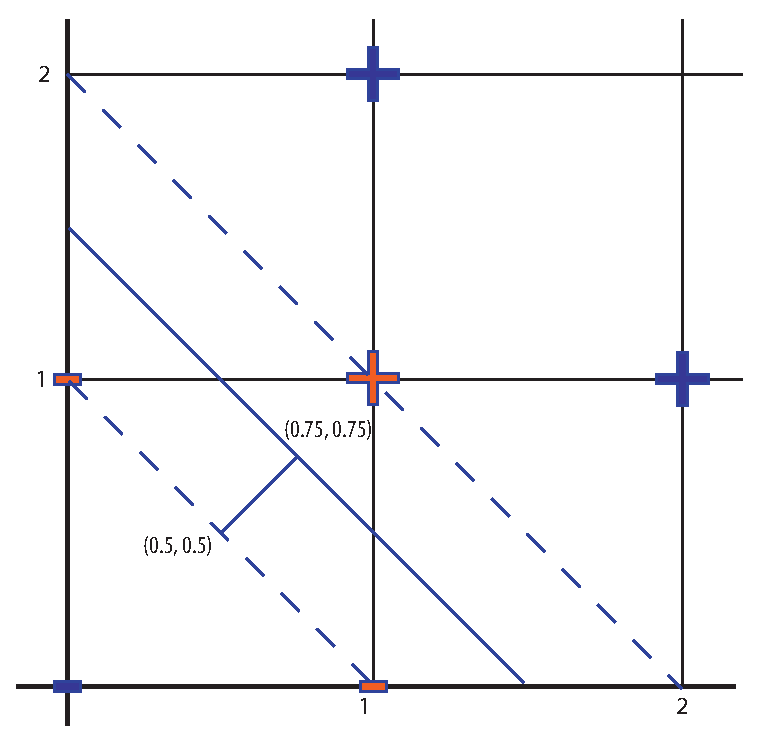
\includegraphics[scale=1]{supportvectors.eps}
\caption{Support vectors, margins, and the optimal separating line.}
\label{fig:vector}
\end{center}
\end{figure}



\item \textbf{2-norm soft margin: }
\begin{enumerate}
\item %a
\end{enumerate}
\end{enumerate}
\end{document}
